\chapter{Operating Systems Developments}
\section{Plan 9 Port to Blue Gene /L and /P}
\subsection{Large Pages}
Blue Gene   processors use software-loaded TLBs. A TLB manages the virtual to physical mapping for a single page, which 
in both Linux and Plan~9 is 4096 bytes. The processors support more than just one page size, in multiples of 4, from 1024 bytes to 1 Gbyte (with a few sizes missing). 
The CNK 
features 1 Mbyte TLBs, and benefits from reduced TLB fault interrupts. 

We extended Plan~9 to support larger TLBs. In order to measure the improvement we used the strid3 benchmark
\begin{figure}[h]
\begin{center}
 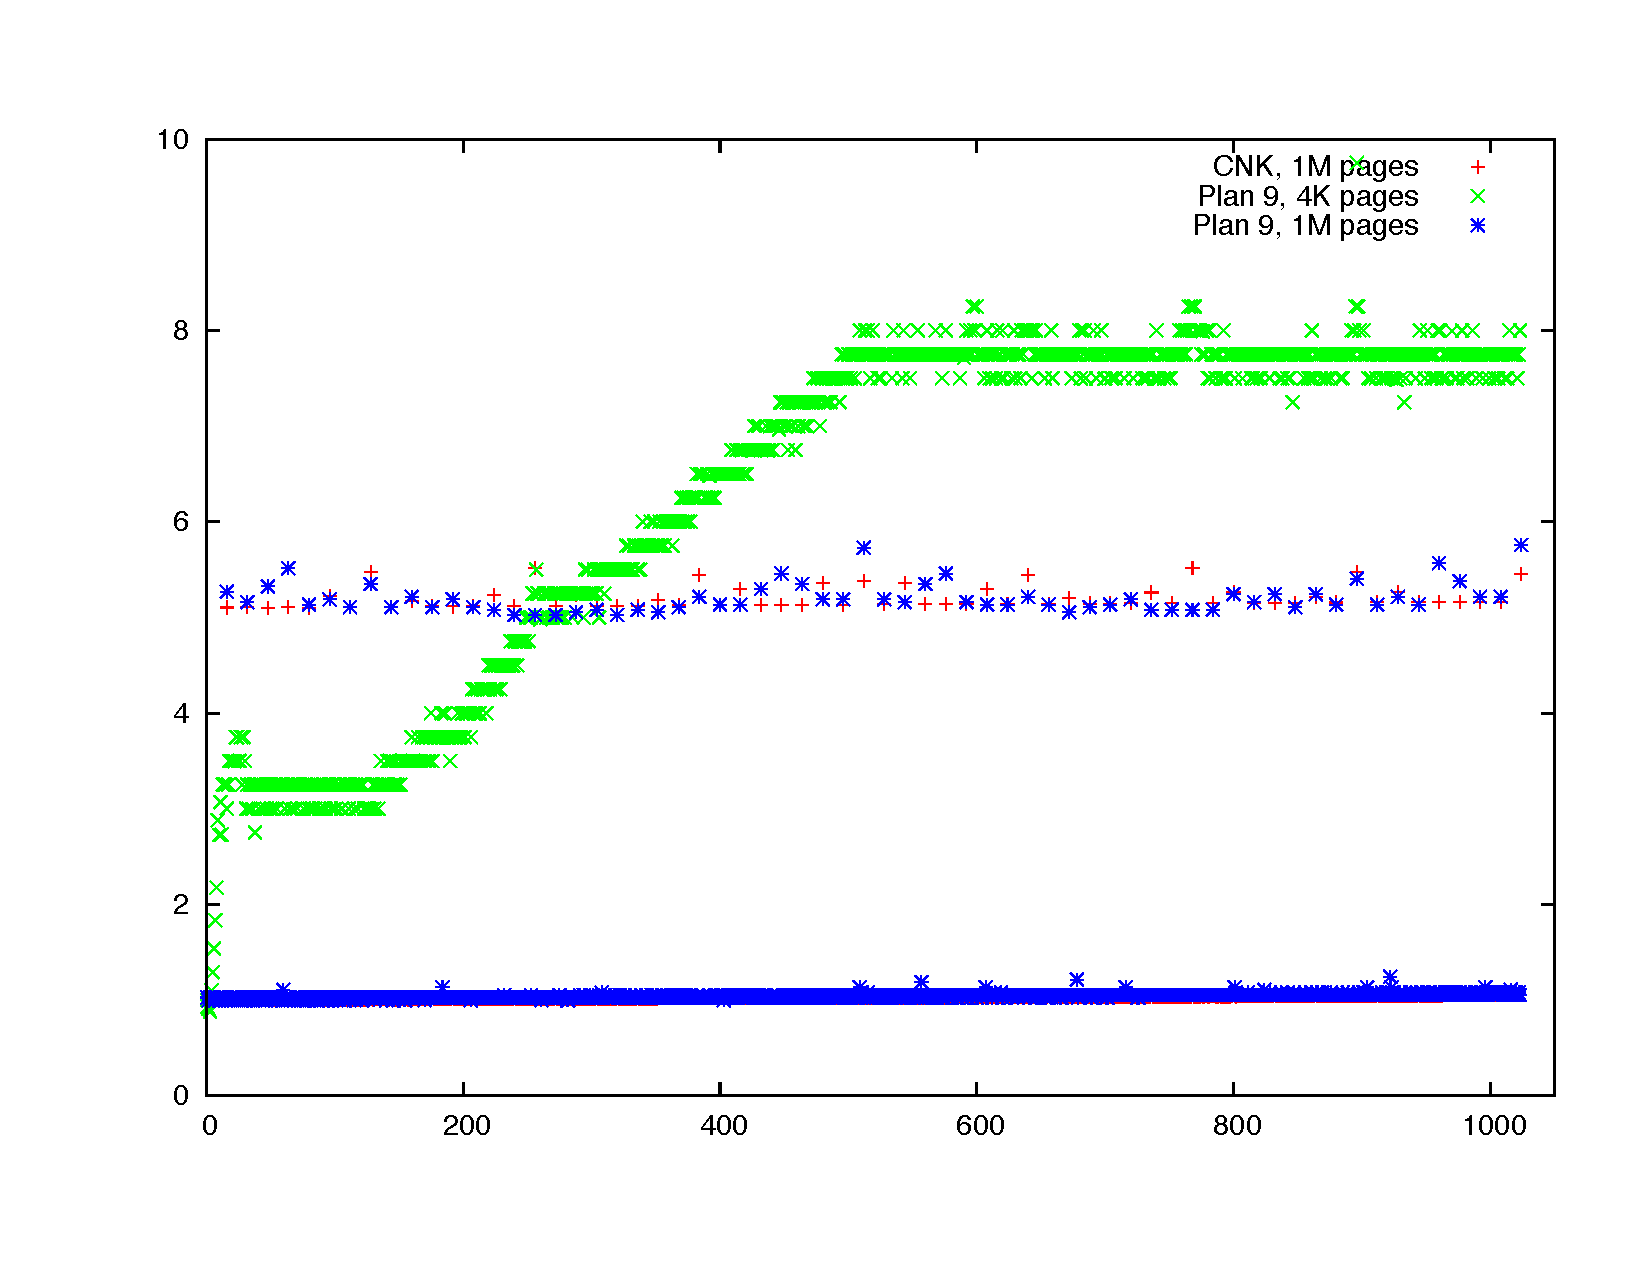
\includegraphics[width=4in]{strid3.pdf}
 \caption{{\bf Result of running strid3 on CNK, Plan 9, and Plan 9 with 1 MByte pages. }}
\label{strid3}
\end{center}
\end{figure}
to show the impact of TLB size upon an application. Shown in Figure \ref{strid3} is the result. Plan~9 is 
eight times slower than the CNK when 4096 byte pages are used. With one Mbyte pages in Plan~9, its 
performance is identical to the CNK. 
The change to Plan~9 to support the larger pages amounted to less than 30 lines of code\cite{DBLP:journals/ife/MinnichM09}. 

\section{Currying and Process-private system calls}
Extensive measurement of the kernel, using the tool developed and described in \cite{plan9trace}, showed
that for read and write system calls a great deal of overhead was repeated for each iteration of the 
call. Two of the biggest overheads are validation of the file descriptor and the read/write pointer and 
length validation. We also found in most cases that the pointers are being reused for each call: it is extremely rare for these parameters to be wrong, yet programs pay the full overhead for checking them 
each time. For the Blue Gene global barrier device, the overhead for the system call was 3.529 microseconds. 

In \cite{currying} we describe the possible approaches to resolving this problem. We developed two 
several extensions to Plan~9 that allowed the kernel to Curry the arguments to the read and write
system calls. The result: the file descriptor and pointer/length information is checked once, and the
result stored in a cache held in the proc struct (per-process information) in the kernel. The per-process structure is 
also extended with a private system call table. When the process makes a private system
call, all the standard checking is skipped and the pre-validated cached values are used instead. This 
new system call path resulted in a 5-fold reduction in overhead, to 729 nanoseconds. 

The Currying and per-process system calls together form a new type of interface to operating system
kernels. 

\subsection{Shared Heap}
Currying reduces the overhead for process-driven operations. It does nothing for interrupt-driven
operations, because interrupts, by design, do not occur in a process context. Page pinning is used 
to resolve this problem on Linux systems: process memory mappings are communicated to the driver
and ``pinned'' into place. Page pinning adds a great deal of code to a kernel; in some cases the
pinning code for (e.g.) Linux is larger than all of Plan~9 itself. 

We implemented a ``shared heap'' model in Plan~9. All process heaps, the kernel, and the drivers 
share a common address space, consisting of the top 1.5 Gbytes of memory. All heap (not text, stack,
or data, 
just heap) is allocated from this shared 1.5 Gbytes of memory. 
A given heap address in a process, kernel, or interrupt handler will
point to the same piece of memory. In contrast, in a standard OS, the same heap address in each 
process points to different memory. Note that a shared heap address space does not imply that 
all the data in the heap itself is shared between all the processes.  
Processes can share parts of the heap, but are typically limited to their own private piece, and 
can not see other processes heap data. 

Processes can easily pass pointers to each other because 
a given heap pointer has the same meaning in every process. Processes can communicate an address 
to the driver for use by the interrupt handler and there is no need for complex pinning, because the 
address has the same meaning in every machine context. 

We further modified the BG/P Torus driver to implement queues on the receive side. As packets are 
received  by the interrupt handler they are directly moved to the queues. 
\footnote{These queues are 
very similar to those provided on the T3D. In the T3D, however, they were implemented in hardware. }
Finally, once the driver and kernel were extended, we created a library to allow processes to 
send from the shared heap and receive into queues in the shared heap. 

Our resulting performance was better than that of the MPI library, even while using 
the kernel for I/O. In fact a simple ping-pong code ran with about 1/3 the latency 
of MPI. Our code was about 100 times smaller than the MPI library. Further, 
the device could be made to work for multiple independent applications, which is not possible
on BG/P hardware if the direct-access MPI libraries are used. We thus showed that if a 
kernel provides the proper abstractions, it is not necessary to run the network device driver
in user memory, as is done today. 

\section{File Systems}
\subsection{Compute Node Caches}

We needed to reduce the load on the file server shared by thousands of
nodes in a Blue Gene Plan 9 cluster. The intent was to execute the caching
mechanisms on the I/O nodes as well as look at spreading them out amongst 
the compute nodes depending on the I/O requirements of a particular 
application.  

Plan 9 had two existing caching mechanisms for 9P file servers: a volatile 
cache controlled by devmnt, and a persistent disk-based cache managed by 
the user-level server cfs.
Both sent the server all 9P requests except reads satisfied by the cache.
Cfs was quickly converted to a ramcfs that used the large memory of a
Blue Gene I/O node instead of a disk, but most 9P traffic still passed
through. A redesign produced fscfs, which breaks the direct link
between its client's 9P transactions and those it makes to the server,
producing a dramatic reduction in traffic seen by the server.

Fscfs is a normal, user-level C application, using the Plan~9 thread
library, libthread, for internal 
concurrency. Like cfs, it is a 9P transducer: it acts as a client to a 
remote 9P file server on one connection, and acts as a 9P server to its 
client on another connection. (Once that connection is mounted in the name 
space, many client processes can share it.) To provide data caching, fscfs 
uses the same strategy as the existing caches: it makes a copy of the data
as it passes through in either direction, and stores it in a local cache. 
Subsequent read requests for the same data will be satisfied from the cache. 
Write requests are passed through to the server, replacing data in the 
cache if successful. Cached data is associated with each active file, but the 
memory it occupies is managed on a least-recently-used basis across the 
whole set of files. When a specified threshold for the cache has been reached, 
the oldest cached data is discarded.

Fscfs maintains a path tree representing all the paths walked in that tree, 
successfully or 
unsuccessfully. A successful walk results in an end-point that records a
handle referring to that point in the server's hierarchy. (Note that 
intermediate names need not have server handles.) If a walk from a
given point failed at some stage, that is noted by a special path value at 
that point in the tree, which gives the error string explaining why the walk 
failed. If a subsequent walk from the client retraces an existing path, 
fscfs can send the appropriate response itself, including failures and walks 
that were only partially successful. If names remain in the walk request 
after traversing the existing path, fscfs allocates a new handle for the new 
path end-point, sends the whole request to the server, and updates the path 
appropriately from the server's response. Remembering failures is a
great help when, for instance, many processes on many nodes are enumerating 
possible names for different possible versions of (say) Python library 
files or shared libraries, most of which do not exist. (It would be more 
rational to change the soft ware not to do pointless searches, but it is not 
always possible to change components from standard distributions.)

Fscfs is just over 2,000 lines of C code, including some intended for future 
use. It has more than satisfied our initial requirements, although much more 
can be done. It aggregates common operations in a general but straightforward 
way. Its path cache is similar to Matuszekps file handle cache in his NFS cache,
and closer to 9P home, some of the subtle cases in handles management in 
fscfs seem to turn up in the implementation of 9P in the Linux kernel, 
where Linux lacks anything corresponding exactly to a 9P handle.

\section{New network communications models}
\subsection{Active Message Support}
As a performance measurement experiment we implemented 
Active Messages in the Torus driver. Our implementation 
of shared heaps, mentioned above, allowed us to do the active message
operation in the torus interrupt handler. The result was an 
ability to perform remote put/get/queue insert at a rate roughly 
three times greater than when MPI was used. 

\subsection{High performance network transport}
\subsection{Network programming models}
Writing or converting applications to make best use of runtimes such
as MPI can be non-trivial: to avoid the synchronization imposed by
matching sends and receives, and barriers, and to overlap
communication to reduce latency, programmers use non-blocking
primitives and asynchronous communication.

In UNIX, a program can read and write on a file descriptor to
communicate with a local device, or a TCP/IP port on a distant
machine, without changing the program text or even recompiling it: IO
through file descriptors is location independent.  The intention
behind developing specialized protocols---the bulk messaging protocol
in particular---and the new messaging kernel interface is to allow HPC
applications to be written in a similar style, but with efficient
transport.  

With IO through file descriptors, if two communicating
processes are on the same node, the system will use cross-domain
references to transfer the data directly; if they are on different
nodes, the sender's data will be passed by reference through the
kernel to the bulk messaging drivers, which will use DMA to transmit
it to memory on the remote node, which will be passed by reference
from the kernel to the receiving process.  File descriptors hide the
protocols used, not just the location.  When debugging on a laptop,
pipes can replace the fancy networks, without changing the program, or
the communication semantics.  It is at least as easy to use as the
naive use of MPI's send/receive, but without imposing a static process
structure, since new processes can be created on demand, and added to
the communication set, in the same way as in network applications.

The primitives are usable both directly by applications and by
supporting services.  For example, we ported to Plan 9 a small
scientific application that used MPI, in which asynchronous
communication had resulted in a complex structure.  We replaced all
MPI calls by calls to a small library using our primitives.  (The
library provides \emph{reduce} and \emph{allreduce} operations, for
instance.)  The revised program is written in a straightforward style,
like a simple network application, as if the communication were
synchronous, but the kernel and its protocol drivers exploit
the potential for concurrency and overlap.  As another example, we
have been experimenting with a small library and associated services
that creates a distributed spanning tree (which can be made
fault-tolerant) to provide multicast and convergecast to support
large-scale computations.

\subsection{Data network basics}
The Blue Gene system provides several data networks.  The IO nodes are
linked by Ethernet, with connections through switches to the outside
world, providing a conventional IP network.  The CPU nodes are
connected by the Torus; and the IO and CPU nodes are linked in a
collective network.  The only path from a CPU node to the outside
(including external file service) is through the collective to an IO
node, and then through the IP network on the Ethernet.  The Ethernet
supports large packets (`jumbo frames').  The collective and Torus,
however, provide only small packets: 256 and 240 bytes of user data
respectively.  On BG/P, compared to BG/L, the Torus has extra DMA
interfaces to the Torus that can automatically fragment messages into
the network's tiny payloads, although the recipient must still
reassemble messages.

The Plan 9 IP stack is completely independent of the MAC layers: a
small \emph{medium} driver connects the bottom of the IP stack to the
files representing the driver for a given MAC level.  For example, the
Ether medium driver opens \texttt{/net/ether0/data}, reads and writes
the file, converting as it does so between the Ether packets the
device expects and IP packets, adding and removing MAC headers, and
invoking ARP as required.  It was a simple task to write specific
medium drivers for each of the Torus and collective networks, just
several hundred lines each.  Note that unlike some other systems on
Blue Gene, Plan 9 therefore does not emulate an Ethernet on either
torus or collective to implement IP. Not only is the MAC-level framing
of IP packets specific to each device, but there is no need for ARP
(which historically has been a problem when attempting to scale to
thousands of nodes).

Raw access (ie, non-IP) to each network is also provided, through
specific device files in the name space, such as
\texttt{/net/torusdata}; in fact, it is the same interface used by the
IP medium drivers.  Applications that use the networks outside IP
often need to send messages larger than the hardware's payload.  We
therefore added a simple fragmentation protocol, allowing messages of
up to 64 kbytes to be exchanged across the network.  The
implementation is about 300 lines, allowing for an implementation
entirely in software on BG/L, and a hybrid implementation on BG/P that
takes advantage on the Torus of support in the DMA subsystem for
fragmentation, using a software header encoding that allows correct
but efficient reassembly at the receiver even when several nodes are
communicating with the same recipient.  Note that combining
fragmentation with IP is worthwhile: the basic IP header is 20 bytes,
and TCP adds 20 more, which is a non-trivial overhead for the tiny
Torus and collective packets.  Fragmentation allows one TCP/IP header
to be used for a large message, which is then fragmented; although
there is overhead in fragment reassembly, the resulting message
traverses the IP stack only once, instead of many packets.

\subsection{Transport protocols}

As noted elsewhere, Plan 9 uses the 9P protocol to implement a range
of system and application services, including distributed services,
such as those provided by the Unified Execution Model.  Unusually for
modern network protocols, 9P is not 9P/IP: it is not expressly an
Internet protocol.  It can use any underlying transport that provides
reliable, sequential (in-order) delivery; the current version of 9P
does not even require the transport to respect 9P message boundaries.
Having implemented an IP network above both Torus and collective
networks, and thus TCP/IP, we could immediately deploy 9P.  The Blue
Gene environment, however, like many supercomputer systems, makes it
easy to experiment with alternative protocol designs and
implementations.  Although the nodes, directly or indirectly, access
resources on outside networks such as file service or graphics
display, much of the communication is intra- and inter-node.
Furthermore, it is easy to change the protocol implementation at all
nodes from run to run, simply as a by-product of rebooting the system.
By contrast, there are many barriers to experimenting with new
protocols on the Internet.  For example, Plan 9 historically had a
reliable datagram protocol, called IL/IP, tuned to the needs of 9P.
It has seen reducing use because on the wider Internet, intervening
routers and firewalls do not recognise the protocol; nor is it easy to
change them to do so.

As well as supporting 9P, which is a reliable point-to-point
conversation between client and server, we wanted to support reliable
messaging between arbitrary pairs of processes (between any nodes).
On Blue Gene, of course, the underlying hardware networks provide just
such reliable delivery, at least in principle, and we had added
fragmentation to allow larger, more expressive messages.  On the other
hand, in the larger context of the project, we were interested in
fault-tolerance, including operation on unreliable or failing
networks.  Furthermore, because of its intended use for a single
application using MPI, the hardware's properties are not quite right
for 9P, or even general inter-process messaging.  Most obviously,
reliability and flow-control are between nodes, not between
collections of processes on those nodes.  Adding multiplexing of
inter-node channels, for example by running IP, requires keeping the
receiver `live' (ie, unblocked) at all times, to prevent the hardware
flow-control from triggering and causing deadlock. Thus, for reliable
communication, the hardware level flow-control is neither necessary
nor sufficient, and flow-control must be added somewhere in the
multiplexing software stack.

Multiplexing, datagram and transport protocols are superficially
straightforward, but typically become burdened with much practical
detail, for connection establishment, error control, flow control, and
congestion control. %\cite{John-Day-Patterns-of-Network-Archictures}
Rather than risk the time to develop a complete protocol from scratch,
we decided to adopt and adapt an existing complete protocol
definition, or more probably a suitable subset of one, limiting the
implementation to just what we needed in the Blue Gene environment.
We needed multiplexed messaging connections for 9P, and reliable but
connectionless messaging for computational work.  The first attempt
was loosely based on the Xpress Transport Protocol,\cite{xtp} which
had the attraction of supporting unreliable and reliable datagrams,
and reliable connections as supersets of each other.  The protocol
essentially microcodes the effects desired by the application level;
thus, a reliable datagram includes one protocol header that declares a
new connection, transfers data into it, requests an acknowledgement,
and closes the connection; a reliable connection instead puts those
operations in the headers of distinct messages, in particular leaving
the connection open after the first message, and taking advantage of
the context thus established to abbreviate subsequent messages.  Plan
9's TCP/IP has 3236 lines for the TCP level, 706 for the IP level, and
some auxiliary code.  By contrast, the XTP prototype had 1740 lines of
code, and needed no IP level, but supported not just TCP-like
connections, but reliable datagrams as well.  Unfortunately,
connection establishment and reset in XTP still seemed overly complex
for this application, requiring message exchanges and timers.  A
second attempt was made (reusing much of the code), inspired by a much
older protocol \emph{delta-t}.\cite{watson1989delta} It was simpler than XTP,
and had a unique, timer-based approach to connection management.
Briefly, in delta-t a logical connection exists between every possible
sender and every possible receiver, but a connection is
quiescent---thus requiring no state on either sender or receiver---if
no message has been sent or received for a specified interval.  The
delta-t designers observed that timers are required to detect time
out, and to provide protection against lost messages on connection
close, but the timers can be used instead to make the connection
messages redundant.  Thus, to use a connection, a process simply sends
a message on it, and the receiver then creates the state for the
connection. After an optional acknowledgement, if no further messages
are received (or the receiving process has no reply), the connection
becomes quiescent and the state is removed. In the original protocol
there are therefore no extra messages for connection establishment or
shutdown, and the protocol can carry a single message efficiently.  An
old quip is that one cannot afford to have (say) TCP/IP connections
between every pair of 65,000 nodes.  With the delta-t approach, the
pair-wise connections (logically) exist but cost nothing, until
messages are actually sent, when the transient state can carry as much
data as needed, reliably, and without extra messaging for connection
establishment.

On the other hand, and currently the primary use, a delta-t connection
can carry 9P traffic between a client and a 9P server. Because the
interface to the protocol (ie, \texttt{/net/pk}) obeys the Plan 9 name
space conventions for networks, applications can use the protocol
instead of TCP/IP without change.

\subsection{Bulk messaging}

On BG/L, the Torus network hardware presented a collection of
memory-mapped FIFOs as its interface, accessed from the processor by
explicit loads and stores.  The BG/P Torus hardware hides that detail
behind a collection of rings of DMA descriptors, and new DMA hardware
moves the data between memory and selected FIFOs.  The hardware goes
much further, however, which required revisiting the software network
interfaces to the Torus.  (The collective networks were unchanged.)
In particular, the hardware provided new DMA operations: \emph{put}
and \emph{remote get}, implemented by special packets interpreted by
the DMA engine.  The Put operation causes the hardware to send an
arbitrarily-large block of memory from one node, across the Torus,
directly into a block of memory on a specified target node.  The
destination address is specified as an offset from a base address in a
table on the remote node, selected by a `counter ID' specified by the
sender.  In the other direction, one node sends a Remote Get packet to
a second node, causing its DMA engine to execute a \emph{Put}
operation.  Usually the target of the Put is the first node, so that
the original message thus gets the relevant data from the second node
efficiently using DMA.

To exploit the BG/P extensions, the Plan 9 Torus driver was extended
to implement a lightweight protocol for bulk messaging. A process
wishing to use bulk messaging opens the file \texttt{/net/torusbig},
and sends and receives messages using write and read system calls. The
first 32 bytes of the data in each read or write is a software header
giving source and destination network addresses, an operation code, a
parameter, and 24 bytes of uninterpreted data for use by the
application.  That is followed by the data of the bulk message itself.
The uninterpreted data might contain values for subaddressing, or
metadata describing the data, but that is up to the application. The
operation code and its parameter are reserved to the protocol
subsystem.

Bulk messaging is a network protocol. Writes and reads are not
matched, let alone synchronised, even in the implementation of the
protocol. A write causes a bulk message to be sent to the destination
node, which is queued until some reader does a read.  The application
data attached to the message might be used to associate requests and
replies in an application level algorithm, perhaps by library code,
but that is outside the messaging protocol.

In the Torus driver, the protocol implementation uses the normal Torus
packet channels, but bulk message control packets are specially
marked, and interpreted by the interrupt handler on the destination
node. A bulk write request sends a Get control message to the
destination. The control message includes the metadata from the
request, and addressing information for the data. If the destination
cannot process the request, it will reply with a Nak. Otherwise, it
will issue a DMA Remote Get request, quoting the addressing
information it was given. The hardware on both source and destination
nodes is programmed to signal an interrupt when the transfer
completes. The sending node marks the bulk request done; the receiver
queues the data to be read. Control packets carry tags to allow
requests to be cancelled, acknowledged, or nak'd if required.

Note that the bulk writer is not required to wait for the transmission
to complete, allowing the usual overlap provided by buffering.  More
subtly, although the transfer is logically a `put' from source to
destination, the \emph{receiving} kernel initiates the transfer using
a DMA Remote Get.  There are several reasons. First, the parameters
for a DMA Put require the sender to specify the correct index in a
table on the \emph{receiver}, and that can only be known by global
convention or prior arrangement (ie, through a previous exchange of
messages), neither of which supports dynamic communication
well. Second, the receiver needs to find the memory to receive the
data, and might be receiving from many other nodes.  Having the
receiver start the transfer allows various forms of flow control.
Most important, however, using DMA Remote Get is more robust against
node failure.  If the sending node fails and stops, the request will
fail or time out.  If the sending node fails and restarts, at worst
the Get request will fetch incorrect data, or receive an error. The
metadata can be used to check the data.  By contrast, if a DMA Put is
used, and a destination node fails and restarts, it is possible that,
without an error being notified, the put will transfer into whatever
memory is addressed at the time by the table index parameter,
corrupting the target node.

\subsection{IO segments}

For initial experiment, we limited messages to 128 KiB, because of
addressing constraints in the system. We did, however, want bulk
messaging to be able to send much larger chunks of data.  Furthermore,
the normal read and write system calls imply copying, which is
obviously inefficient.  We changed the system to allow both
restrictions to be removed, by solving a more general problem. We
added a simple form of cross-domain reference.

A process can attach a special type of segment intended to be used for
IO.  The segment is backed by physically-contiguous memory, usable by
hardware DMA.  Inspired by the x-kernel \cite{hutchinson1991x}, fbufs
\cite{fbufs}, and System 360's LOCATE mode, two new system calls were
added:


\begin{center}
      Message readmsg(int fd, uint iolimit)

      int writemsg(int fd, Message m)
\end{center}

Like the read system call, readmsg fetches data from the file denoted by file descriptor fd,
but instead of having the user provide a buffer address, readmsg returns a Message value
that refers to the data read (ie, the buffer address), and any associated metadata (eg, source address). Similarly, writemsg accepts a Message value instead of a single buffer address.
The data address in the Message can be an ordinary address in the process.
but it can also be a reference to an IO segment.
Such references can be passed between user process and device driver through the kernel.
There are primitives to manage the memory in an IO segment.

In the HARE implementation on BG/P, IO segments and the system calls are restricted to use with particular devices, specifically the Torus.
Since then, however, we have revised and extended the scheme in the context of the 64-bit NIX work,
to handle IO to arbitrary devices, and support interprocess communication.


\section{Kittyhawk Kernels and VMM}

Supercomputers and clouds both strive to make a large number of 
computing cores available for computation. 
However, current cloud infrastructure does not yield the performance 
sought by many scientific applications. A source of the performance 
loss comes from virtualization and virtualization of the network in 
particular. 
Project Kittyhawk~\cite{kh-sciencecloud} was an undertaking at IBM Research 
to explore the use of a hybrid supercomputer software infrastructure
on top of a BlueGene/P which allows direct hardware access to the 
communication hardware for the necessary components while providing 
the standard elastic cloud infrastructure for other components.

Beyond the enabling infrastructure for cloud provisioning and dynamic
boot of multiple images across compute nodes within a single BG/P
allocation, the Kittyhawk team also ported a Linux compute node
implementation complete with an Ethernet interface to the high-performance
collective and torus networks~\cite{kh-systemsjournal}.  
This allowed Linux applications to run unmodified on Blue Gene compute 
nodes without incurring the performance 
overhead of reflecting sockets and I/O operations thorugh user space
helpers as in ZeptoOS.  It also enabled more conventional storage solutions
including SAN and NAS to be extended into the compute node network for
I/O intensive solutions.  While the Kittyhawk Linux kernel provided this
Ethernet interface, it also provided an API allowing the allocation of
torus channels directly to high performance applications which knew how to
interact with them allowing even greater degrees of performance and flexibility.
These allocated application channels co-existed with the kernel-space channels
providing a good hybrid trade off between system provided networking and
OS bypass.

The Kittyhawk environment was not limited to Linux kernel targets.  
It also supported execution of the L4 microkernel operating system.  
In addition to providing an alternative execution platform for applications,
the L4 Kittyhawk port also supported a virtual machine monitor which could
be used to further virtualize the BG/P nodes and network providing additional
protection in cloud deployment environments.

The Kittyhawk infrastructure, the linux kernel patches, and the L4 kernel
and virtual machine monitor have all been released as open source and are
available from http://kittyhawk.bu.edu.
